Since the Higgs boson was first observed in 2012 by the CMS and ATLAS collaborations~\cite{Aad:2012tfa, Chatrchyan:2012xdj, Chatrchyan:2013lba}, characterizing its properties has remained one of the highest priorities of the LHC research program. 
The Standard Model predicts values for many properties of the Higgs boson, including the strength of its coupling to the other elementary particles.
Physics beyond the Standard Model, such as mechanisms of mass generation other than spontaneous symmetry breaking, could modify these coupling strengths. 
Consequently, precise measurements of the Higgs boson's coupling to elementary particles are of great interest: any deviation from the Standard Model prediction could be indicative of the presence of new physics.
%
\subsection{The Top Quark Yukawa Coupling}
The coupling of the Higgs boson to the top quark, called the top quark Yukawa coupling, is of particular interest from a theoretical standpoint.
Specifically, the top quark Yukawa coupling can help give an indication about the scale of new physics~\cite{why_care_top_yukawa}.

A primary means of constraining the top quark Yukawa coupling is through the measurement of the \ttH production cross section, which is proportional its square:
\begin{equation}
\sigma_{\ttH} \propto y_{\text{t}}^2.
\end{equation}
The dominant tree-level diagram for \ttH production is shown in Fig.~\ref{fig:tth_feynman}.
\begin{figure} [htbp!]
    \centering
    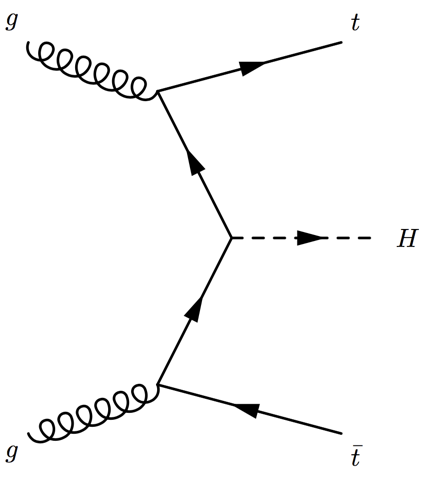
\includegraphics[width=0.4\linewidth]{figures/tth/tth_feynman.png}
    \caption{Tree-level production of a Higgs boson in association with a top quark-antiquark pair.}
    \label{fig:tth_feynman}
\end{figure} 

This is in fact the best method of \emph{directly} constraining the top quark Yukawa coupling at the LHC.
Indirect constraints on $y_\text{t}$ come from measurements of Higgs boson production via gluon fusion and \Hgg decay, both of which proceed primarily through a top quark loop, as in Fig. ~\ref{fig:hgg_feynman}.
However, these constraints are indirect because they make the assumption that no other BSM particles also contribute to the loops. 

Complementary methods of constraining $y_\text{t}$ include extraction from the shapes of kinematic distributions in \ttb events~\cite{CMS:2020qzr}, reporting a measured value of $y_\text{t} = 1.16^{+0.24}_{-0.35}$.
This measurement does, however, rely on the aforementioned assumptions about the \Hgg branching ratio, and is said to be an indirect constraint on the top Yukawa coupling.
%The uncertainty on $y_\text{t}$ is more than a factor of 2 less than that obtained with a measurement of \ttH (\Hgg)\footnote{One caveat is that the \ttH (\Hgg) result does not quote an actual value of $y_\text{t}$, but rather the \ttH cross section, which is proportional to the square of $y_\text{t}$.}, but does not rely on assumptions about the \Hgg branching ratio.

\subsection{Landscape of \ttH Measurements}
The first observation of the \ttH process was reported in 2018 by the CMS experiment~\cite{Sirunyan:2018hoz}, using 36 \fbinv of data from pp collisions at $\sqrt{s} = 13$ TeV.
The first observation of \ttH production in a single H decay channel (\Hgg) was reported by the CMS collaboration~\cite{tth_observation}, with the ATLAS collaboration reporting a similar result shortly after~\cite{Aad:2020ivc}.
The CMS observation of \ttH (\Hgg) is detailed in the following sections of this thesis.



%\subsection{\ttH~Production as a Probe of the Top Quark Yukawa Coupling}
